\documentclass[10pt, twocolumn]{article}

%math
\usepackage{amsmath}
\usepackage{amssymb}
\usepackage{mathtools}
%logic
\usepackage{pgffor}
\usepackage{ifthen}
%science
\usepackage{siunitx}
\usepackage[version=4]{mhchem}
%language
\usepackage[english]{babel}
%formatting
\usepackage[a4paper, portrait, margin=1in]{geometry}
\usepackage{cuted}
\usepackage[small]{titlesec}
\usepackage[hidelinks]{hyperref}
\usepackage{parskip}
%images and plots
\usepackage{graphicx}
\usepackage[justification=centering]{caption}
\usepackage{subcaption}
\usepackage{float}
\usepackage{pgf}
\usepackage{import}
\usepackage{jsonparse}
%tables
\usepackage{booktabs}
\usepackage{makecell}
%citation, quatation and lists
\usepackage[style=numeric,maxcitenames=2,sorting=none,doi=false,
url=false,isbn=false,eprint=false]{biblatex}
\usepackage[noabbrev,nameinlink]{cleveref}
\usepackage{csquotes}
\usepackage[nottoc]{tocbibind}
\usepackage{acro}


%setup plugins
\addbibresource{literature.bib}

\captionsetup{justification=centering}
\hypersetup{colorlinks=true,linkcolor=blue}


\DeclareSIUnit\angstrom{\text {Å}}
\DeclareSIUnit\bar{bar}
\sisetup{
	range-phrase = { to }
}

% Custom \citeauthoryear command with hyperref -> Rost et al. (2019) 
\DeclareCiteCommand{\citeauthoryear}
{\boolfalse{citetracker}%
\boolfalse{pagetracker}%
\usebibmacro{prenote}}
{\ifciteindex
{\indexnames{labelname}\indexfield{year}}
{}%
\printtext[bibhyperref]{%
    \printnames{labelname}%
    \setunit{\addspace}%
    \printtext{(}%
    \printfield{year}%
    \printtext{)}}}
{\multicitedelim}
{\usebibmacro{postnote}}

%  setup custom commands
\newcommand{\imcite}[2][]{From \cite[#1]{#2}.}
\newcommand{\imcitetwo}[2][]{Based on \cite[#1]{#2}.}
\newcommand{\integral}[4]{\int_{#1}^{#2} #3 \mathrm{d} #4}
\newcommand{\derivative}[2]{\frac{\mathrm{d}}{\mathrm{d} #1} #2}

%import json
\JSONParseFromFile{\tasktwo}{../plots/task_2_data.json}
\JSONParseValue[store in = \taskTwoSlope]{\tasktwo}{slope}
\JSONParseValue[store in = \taskTwoEnergy]{\tasktwo}{donor_energy}
\JSONParseValue[store in = \taskTwoSlopeOne]{\tasktwo}{mobility_1}
\JSONParseValue[store in = \taskTwoSlopeTwo]{\tasktwo}{mobility_2}
\JSONParseValue[store in = \taskTwoSlopeThree]{\tasktwo}{mobility_3}

\JSONParseFromFile{\taskthree}{../plots/task_3_data.json}
\JSONParseValue[store in = \taskThreeSlope]{\taskthree}{slope}
\JSONParseValue[store in = \taskThreeEnergy]{\taskthree}{donor_energy}
\JSONParseValue[store in = \taskThreeSlopeOne]{\taskthree}{mobility_1}
\JSONParseValue[store in = \taskThreeSlopeThree]{\taskthree}{mobility_3}




% Document
\begin{document}
\pagenumbering{arabic}
\begin{strip}
	\begin{centering}
	\huge Semiconductor Physics Laboratory \RN{1}\\
	\LARGE A4: Free Charge Carriers\\
	\vspace{0.35cm}
	\normalsize Simon Legtenborg, 3773994 \\ 
	\normalsize Experiment conducted on 18.12.2024 \\
	\vspace{1cm}
\end{centering}

\end{strip}
Die Breite einer Spalte beträgt: \the\columnwidth
\paragraph{Abstract}
This lab report examines fabrication of a \ce{ZnO} thin film on a c-sapphire
substrate using \acs*{pld}.
The fabricated \ce{ZnO} sample and a \ce{SrTiO3} thin film were characterized using
\acs*{rheed}.



\section{Free Carrier Statistics}
In order to draw conclusions about material properties by analyzing
the temperature dependence of the charge carrier density,
free carrier statistics and especially the influence of doping shall be
discussed.
\subsection{Charge Carrier Density}
The number of electrons per volume in the conduction band $n$ is
determined by the following expression:
\begin{equation}
	n=\int _{E_{\mathrm{C}}}^{\infty} D_{\mathrm{e}}(E)
	f_{\mathrm{e}}(E)\, \mathrm{d}E.
	\label{eq:n_int}
\end{equation}
In this equation, $E_{\mathrm{C}}$ represents the minimum energy level of
the conduction band. The function $D_{\mathrm{e}}(E)$ describes
the density of electronic states at a given energy $E$, while
$f_{\mathrm{e}}(E)$ is the statistical distribution function.
For electrons, this function is the Fermi-Dirac distribution that can be
defined with $E_\mathrm{f}$ as the Fermi-energy, $\mathrm{k}$ as the
Boltzmann constant and $T$ as temperature:
\begin{equation}
	f_{\mathrm{e}}(E)
	=\frac{1}{\exp((E-E_{\mathrm{F}})/(\mathrm{k}T))+1}.
\end{equation}
In order to solve the integral in \cref{eq:n_int}, a functional
expression for the density of states is required.
A suitable approximation that utilizes the effective electron mass
$m^*_\mathrm{e}$ are
parabolic band edges which originates from the free-electron gas:
\begin{equation}
	D(E)=\frac{1}{2\pi^2}
	\left( \frac{2m^*_\mathrm{e}}{\hbar^2} \right)^{3 / 2} \sqrt{E}.
	\label{eq:para_band_edges}
\end{equation}
By substituting \cref{eq:para_band_edges} into \cref{eq:n_int} and applying
the transformations $\eta=E_\mathrm{F}-E_\mathrm{C}$,
$x = (E-E_\mathrm{C}) / (\mathrm{k} T)$, the integral can be brought into
the following form:
\begin{align}
	n            & = N_\mathrm{c} \frac{2}{\sqrt{\pi}}
	\int_{0}^{\infty} \frac{\sqrt{ x }}{1+\exp(x-\eta / (\mathrm{k}T))} \,
	\mathrm{d}x \label{eq:n_int_2},                                        \\
	N_\mathrm{c} & = 2 \left( \frac{2 \pi m^*_\mathrm{e} \mathrm{k}T}{h^2}
	\right)^{3 / 2}.
\end{align}
\Cref{eq:n_int_2} represents a form of the Fermi-Dirac integral
$F_{1 /2}(\eta  / (\mathrm{k}T))$.
For $0 \gg \eta$,
this function can be approximated by $F_{1 /2}(\eta  / (\mathrm{k}T))
	\simeq \exp(\eta /(\mathrm{k}T))$.
Semiconductors that fulfill this requirement all called degenerate.
With that approximation, the free carrier density can be expressed as
a function of the Fermi-energy:
\begin{equation}
	n	= { N_{\mathrm{C}} }\exp\left( \frac{E_{\mathrm{F}}
		-E_{\mathrm{C}}}{\mathrm{k_B}T} \right).
	\label{eq:n}
\end{equation}
The same procedure can be applied in an analogous way for holes instead of
electrons.
Let $p$ be the number of holes per volume in the valence band,
one finds with similar assumptions:
\begin{align}
	p            & = N_\mathrm{V} \exp
	\left( - \frac{E_{\mathrm{F}}-E_{\mathrm{V}}}{\mathrm{k}T} \right)^{3 / 2}
	\label{eq:p},                                        \\
	N_\mathrm{V} & = 2 \left( \frac{2 \pi m^*_\mathrm{h}
		\mathrm{k}T}{h^2} \right).
\end{align}

\subsection{Intrinsic Conduction}
For an ideally pure semiconductor, only valence-band electrons
can exite into the conduction band.
This leads to the following charge neutrality condition:
\begin{equation}
	n = p.
\end{equation}
With this additional constraint, a formula for the free
carrier concentration can be found that only depends on the
band gap $E_\mathrm{g} = E_\mathrm{C} - E_\mathrm{V}$ by
substituting \cref{eq:n} and \cref{eq:p}
into the root below:
\begin{align}
	p & = n = \sqrt{n^2} = \sqrt{n \cdot p} \notag \\
	  & =\sqrt{ N_{\mathrm{V}}N_{\mathrm{C}} }
	\exp\left( -\frac{E_{\mathrm{g}}}{2\mathrm{k}T} \right).
\end{align}

\subsection{Donors and Acceptors}
\begin{figure*}
	\centering
	\includegraphics[width=0.6\linewidth]{../assets/energy_level.png}
	\caption{Energetic position of various donors and acceptors
		for silicon. \imcite{grundmann}}
	\label{fig:energy_level}
\end{figure*}

The conductivity of a semiconductor can be altered using
point defects.
This process is called doping.
If the conductivity is determined by holes, the material is
called p-type.
If the conductivity is determined by electrons, the material
is called n-type.

\paragraph{Donors} are point defect atoms that are incorporated into the crystal
lattice and dispose an additional electron after satisfying all
lattice bonds.
For group-$\mathrm{IV}$ semiconductors, group-$\mathrm{V}$ elements
are donors.
This extra electron is bound to the atom via Coulomb interaction,
which is a result of the higher charge of the donor's core.
The energy level of this electron can be estimated by assuming
energetically rescaled hydrogen orbitals.
This rescaling originates from the effective electron mass and
the screening of the coulomb interaction by the dielectric constant
of the material.
The absolute energetic position of the bound electron is
$E_{\mathrm{D}}=E_{\mathrm{C}}-E_{\mathrm{D}}^{b}$ with
\begin{equation}
	E_{\mathrm{D}}^{b}=
	\frac{1}{\epsilon_{\mathrm{r}}^{2}}
	\frac{m_{\mathrm{e}}^{*} e^{4}}{2(4\pi\epsilon_{0}\hbar)^{2}}.
\end{equation}
Energetic positions of various donors are displayed in
\cref{fig:energy_level}.
Similar to intrinsic conduction, the additional electrons have a
finite probability to shift into the conduction band
(they donate an electron) and
can therefore be used for n-type doping.
The probability for an electron to occupy the bound state $f^0$
(where '$0$' indicates that the donor is neutral) can be expressed
by the Fermi-Dirac distribution.
The probability for an electron to not occupy the bound state $f^+$
(where '$+$' indicates that the donor is ionized) can also be
determined:
\begin{align}
	f_{0} & =\frac{1}{1+\frac{g_{+}}{g_{0}}\exp\left(
	\frac{E_{\mathrm{D}}-E_{\mathrm{F}}}{\mathrm{k}T}\right)},  \\
	\label{eq:fplus}
	f_{+} & =(1-f_{0})=\frac{1}{1+\frac{g_{0}}{g_{+}}\exp\left(
		\frac{E_{\mathrm{F}}-E_{\mathrm{D}}}{\mathrm{k}T} \right)}.
\end{align}
Note that the degeneracy of the states impact the distribution.
A neutral donor has a degeneracy of $g^0=2$, since the bound
electron can take two spin states, the degeneracy of the
ionized donor is simply $g^+=1$.

Either the electron occupies the bound state or it shifts into the
conduction band.
Let $N_\mathrm{d}$ be the donor concentration, $N_\mathrm{d}^0$ the
number of neutral donors and $N_\mathrm{d}^+$ the number of ionized donors.
One finds the following relations:
\begin{align}
	N_{\mathrm{D}}     & =N_{\mathrm{D}}^{+}+N_{\mathrm{D}}^{0},        \\
	N_{\mathrm{D}}^{0} & \simeq N_{\mathrm{D}}f_0                             \\
	\label{eq:ndplus}
	N_{\mathrm{D}}^{+} & \simeq N_{\mathrm{D}}(1-f_{0}) =N_{\mathrm{D}}f_{+}.
\end{align}

\paragraph{Acceptors} are point defect atoms that are incorporated
into the crystal
lattice and lack one binding electron.
They are able to borrow (accept) an electron from the valence band.
For group-$\mathrm{IV}$ semiconductor, elements from group-$\mathrm{III}$
can be used as acceptors.
The energetic considerations are similar to those of donors.
The energy level of an electron that is bound to the acceptor can be
expressed
$E_{\mathrm{A}}=E_{\mathrm{V}}+E_{\mathrm{A}}^{b}$,
where $E_\mathrm{A}^b$ can be represented by rescaled
hydrogen orbitals.

These levels are also displayed in \cref{fig:energy_level}.
The acceptor concentration $N_\mathrm{A}$ can be separated into
the number per volume of ionized acceptors $N_\mathrm{A}^-$ and neutral
acceptors $N_\mathrm{A}^0$, such that the relation
$N_{\mathrm{A}}=N_{\mathrm{A}}^{0}+N_{\mathrm{A}}^{-}$ holds.
Again the probability of finding an electron bound to an acceptor $f$ is
equal to the probability of a hole shifted from the acceptor to the
valence band and can be modelled by a Fermi-Dirac-distribution:
\begin{equation}
	f = \frac{1}{1+\hat{g}_{\mathrm{A}}\exp\left( -
	\frac{E_{\mathrm{F}}-E_{\mathrm{A}}}{\mathrm{k}T} \right)}.
\end{equation}
In this case, the ratio of the acceptor state degeneracies
$\hat{g}_\mathrm{A}$ are nontrivial and need to be considered in detail.

\subsection{Charge Neutrality Condition}
Since donors and acceptors offer additional electrons or holes, the charge neutrality 
condition needs to be modified:
\begin{equation}
	n = p -\sum_i N_{\mathrm{A}i}^- + \sum_j N_{\mathrm{D}j}^+.
	\label{eq:charge_neutrality}
\end{equation}
\Cref{eq:charge_neutrality} can be used to get an implicit functional dependence $f(n,T)$.
A simple example is a material that is doped by only one donator material.
By using \cref{eq:ndplus} and additionally assume sufficient low
temperatures, intrinsic conduction can be neglected and the charge
neutrality condition is reduced to $n = N_\mathrm{D}^+=N_\mathrm{D} f_+$.
Substituting \cref{eq:n} and \cref{eq:fplus} results in:
\begin{align}
	\notag
	n     & =\frac{N_{\mathrm{D}}}{1+\hat{g}
		\exp\left( \frac{E_{\mathrm{F}}-E_{\mathrm{C}}}{\mathrm{k}T} \right)
	\exp\left( \frac{E_{\mathrm{C}}-E_{\mathrm{D}}}{\mathrm{k}T} \right)}                   \\
	\notag
	      & =\frac{N_{\mathrm{D}}}{1+ \hat{g}n /N_{\mathrm{C}}\cdot
	\exp\left( \frac{E_{\mathrm{C}}-E_{\mathrm{D}}}{\mathrm{k}T} \right)}, \label{eq:n_quad} \\
	      & =\frac{N_{\mathrm{D}}}{1+n / n_{1}},                                             \\
	n_{1} & =	\frac{N_{\mathrm{C}}}{\hat{g}}
	\exp\left( -\frac{E_{\mathrm{D}}^{b}}{\mathrm{k}T} \right)
\end{align}
\Cref{eq:n_quad} is a quadratic equation in terms of $n$ and thus
analytically solvable.
This leads to an explicit temperature dependence that can be approximated
for low and high temperature. 
\begin{equation}
	\label{eq:n_T}
	n = \frac{2N_{\mathrm{D}}}{1+\left( 1+4\hat{g} \frac{N_{\mathrm{D}}}{N_{\mathrm{C}}}
	\exp\left( \frac{E_{\mathrm{D}}^{b}}{\mathrm{k}T} \right) \right)^{1/2}},
\end{equation}
\begin{align}
	\label{eq:n_T_approx_low}
	n & \simeq \sqrt{ \frac{N_{\mathrm{D}}N_{\mathrm{C}}}{\hat{g}} }
	\exp\left( \frac{-E_{\mathrm{D}}^{b}}{2 \mathrm{k}T} \right) & \mathrm{k}T\ll 
	E_{\mathrm{D}}^{b} \\
	\label{eq:n_T_approx_high}
	n & \simeq N_{\mathrm{D}} & \mathrm{k}T\gg E_{\mathrm{D}}^{b}
\end{align}

\begin{figure}
	\centering
	\includegraphics[width=0.75\linewidth]{../assets/charge_carrier_density_temperature.png}
	\caption{Charge carrier density as a function of temperature for 
	silicon doped with phosphor. \imcite{grundmann}}
	\label{fig:carrier_temperature}
\end{figure}
$n(T)$ is visualized in \cref{fig:carrier_temperature}.
Note that intrinsic conduction cannot be neglected for sufficient high
temperatures.
\section{Hall effect}
\begin{figure*}
	\centering
	\includegraphics[width=0.8\linewidth]{../assets/hall_geometry.png}
	\caption{Schematic structure for Hall effect measurements.
		\imcite{grundmann}}
	\label{fig:hall}
\end{figure*}
The geometrical arrangement required for Hall effect measurements
is displayed in \cref{fig:hall}.
A magnetic field $\mathbf{B}=B \cdot \hat{z}$ penetrates
a semiconductor sample.
A current $\mathbf{j}$ is flowing along the $x$-direction inside the sample 
as a response to an external electric field $\mathbf{E}=E_x \cdot \hat{x}$.
Due to the magnetic force, the electrons are deflected and a current in
$y$-direction establishes until the resulting electric force in $y$-direction
fully compensates the magnetic force.
The system equilibrates for $j_y=0$.

To describe the system in detail for one majority charge carrier, one can use the 
equation of motion from relaxation time approximation:
\begin{equation}
	m^{*} \frac{\mathbf{v}}{\tau}=q(\mathbf{E}
	+\mathbf{v}\times \mathbf{B}).
\end{equation}
In this equation, $m^{*}$ is the effective mass of the charge carrier, $\mathbf{v}$ the
average electron velocity and $\tau$ the relaxation time constant.
With $\mathbf{j}=nq\mathbf{v}$ and the resistivity tensor $\hat{\rho}$, 
this vector equation can be brought into a linear transformation of the form
$\mathbf{E}=\hat{\rho}\mathbf{j}$ or more explicit:
\begin{equation}
	\label{eq:mej}
	\begin{pmatrix}
		E_{x} \\
		E_{y} \\
		E_{z}
	\end{pmatrix}
	=
	\begin{pmatrix}
		\frac{m^{*}}{\tau nq^{2}} & - \frac{B_{z}}{nq}        & 0                         \\
		\frac{B_{z}}{nq}          & \frac{m^{*}}{\tau nq^{2}} & 0                         \\
		0                         & 0                         & \frac{m^{*}}{\tau nq^{2}}
	\end{pmatrix}
	\begin{pmatrix}
		j_{x} \\
		j_{y} \\
		j_{z}
	\end{pmatrix}.
\end{equation}
The system equilibrates for $\mathbf{j} = j_x \cdot \hat{x}$ and with \cref{eq:mej}, the following
relationship holds true: $E_{y} = B_{z} / (nq) j_{x} = R_{\mathrm{H}}B_{z}j_{x}$.
This leads to an expression for the carrier density $n$ using directly measurable quantities.
\begin{align}
	R_{\mathrm{H}}&=\frac{1}{nq}=\frac{E_{y}}{j_{x}B_{z}}\\
	n&=\frac{j_{x}B_{z}}{E_{y}q}
\end{align}

Now we want to find an expression for the mobility.
\begin{equation}
	\begin{pmatrix}
		E_{x} \\
		E_{y} \\
		E_{z}
	\end{pmatrix}
	=\begin{pmatrix}
		\mu_\mathrm{H}^{-1} & -B_{z}              & 0                   \\
		B_{z}               & \mu_\mathrm{H}^{-1} & 0                   \\
		0                   & 0                   & \mu_\mathrm{H}^{-1}
	\end{pmatrix}
	\begin{pmatrix}
		v_{x} \\
		v_{y} \\
		v_{z}
	\end{pmatrix}
\end{equation}
The hall mobility in this equation is defined as $\mu_{\mathrm{H}}=\frac{q\tau}{m^{*}}$.
To see why this is useful, first, think of the limit $B_{z}\to 0$.
Then, electric field and velocity indeed follow the relation $\mathbf{v}=\mu_{\mathrm{h}}\mathbf{E}$.
Second with $\mathbf{v}=\mu_{\mathrm{h}}\mathbf{E}$ one can easily see that
$v_{x} = \mu_{\mathrm{H}}E_{x}$ and $E_{y}=B_{z}v_{x}=B_{z}\mu_{\mathrm{H}}E_{x}$.
Therefore we find the following equation for $\mu_\mathrm{H}$:
\begin{equation}
	\mu_{\mathrm{H}}=\frac{E_{y}}{B_{z}E_{x}}
\end{equation}

\section{Results and Discussion}
\subsection{Length Calibration}

\begin{figure*}
	\centering
	\includegraphics[width=0.7\linewidth]{../plots/calibration.pdf}
	\caption{Silicon grid pattern for calibration.}
	\label{fig:calibration}
\end{figure*}

The initial task involved calibrating the instrument's length scale with a calibration grid.
\Cref{fig:calibration} displays the silicon grid pattern
used for calibration.
The orange dots indicate points used to assess the grid's periodicity.

Using the picture, the distances between adjacent points have
been calculated and averaged, whereby an average length of
$d_{\mathrm{sem}}=\qty{10.1 \pm 0.5}{\micro\meter}$ was determined.
The manufacturer of the silicon grid provides a periodicity length of
$d_{\mathrm{grid}}=\qty{9.87\pm 0.05}{\micro\meter}$.
This minor deviation can be corrected using a linear
correction function $d = \alpha d^*$, where $d$ is the calibrated
distance, $d^*$ the measured distance and
$\alpha=d_{\mathrm{grid}} /d_{\mathrm{sem}} = \num{0.977}$.
This calibration ensures that subsequent measurements are accurate and
reliable.

\subsection{Investigation of an unknown semiconductor sample}
\paragraph{SED and BSE}
The next task of the lab course was to investigate an unknown sample
that exhibits artifically created structures, see \cref{fig:sample_0}.
The pictures were made in the vicinity of a crossing
point on which three vertical and three horizontal lines intersect.

With the help of different detector modes, it is possible to observe
different material properties.
The first picture, see \cref{subfig:sample_0_sed}, displays a recording
with an SED detector to obtain information about the sample's topography.
Surfaces of the same gray scale should have the same slope because of the
dependency $\delta_\mathrm{SE} \simeq \cos(\theta)$.
Horizontal and vertical grooves are visible, that were probably
fabricated by nanolithography.
At the intersections of the individual lines, additional structures can
be found.
Irregular chunks of crystallites can be seen, which indicate
some kind of crystal growth or residues from nanolithography.

The second and the third picture, see
\crefrange{subfig:sample_0_bsd_full}{subfig:sample_0_bsd_45}, display two
recordings captured with a BSD detector.
Both images have a lower resolution due to the larger area of
\ac{be}-interaction compared to \ac{se}-interaction.

\Cref{subfig:sample_0_bsd_full} illustrates an intensity
distribution where the signals from all BSD detectors have been combined.
The picture displays a clear intensity contrast between the large
homogeneous areas and the line bundles, therefore indicating a material
contrast.
The crystallites have a similar intensity as the large areas, so they
could originate from the same material.

\Cref{subfig:sample_0_bsd_45} presents a similar image, created by
combining signals from variously positioned detectors to simulate the
perspective of a detector positioned at the azimuthal angle of
\qty{45}{\degree} (at the top right of the image).
Differences are visible between the two BSD recordings: The right
half of the vertical lines and the upper half of the horizontal lines
are significantly darker than their opposite area.
Reason for this are no further material contrasts but rather the surface
topography and the position of the detector.
To be more precise, the side walls of the grooves are blocking the signal and
thus preventing the electrons	to reach the detector.

\paragraph{Distance calculation}
In \cref{subfig:sample_0_sed} there are also four distances labeled.
These distances are listed in \cref{tab:distances}.

\begin{table}[h]
	\centering
	\begin{tabular}{cccc}
		\toprule
		label & $d^*$ in \unit{\micro\meter} & $d$ in \unit{\micro\meter} \\
		\midrule
		1     & \num{3.0}                    & \num{2.93}                 \\
		2     & \num{4.76}                   & \num{4.65}                 \\
		3     & \num{3.04}                   & \num{2.97}                 \\
		4     & \num{2.59}                   & \num{2.53}                 \\
		\bottomrule
	\end{tabular}
	\caption{Characteristic distances of the sample.}
	\label{tab:distances}
\end{table}

\paragraph{EDX}
To get a better understanding of the sample's composition, one can
conduct an \ac{edx} spot analysis experiment.
In this lab course, three different spots, see \cref{subfig:edx_spots},
were chosen for two different electron energies:
\qty{10}{\kilo \electronvolt}
and \qty{20}{\kilo\electronvolt}.

The X-ray spectra for electrons with a kinetic energy of
\qty{10}{\kilo\electronvolt} for the selected spots are shown
in \crefrange{subfig:10kV_1_spectrum}{subfig:10kV_3_spectrum}.

The peak positions allow identification of the elements \ce{Ga},
\ce{As}, and \ce{Si}.
The corresponding elemental concentrations are evaluated with the help
of the data analysis program associated with the electron microscope and
are listed in \cref{tab:edx_1}.

The measurements of the first spot show that \ce{Ga} and \ce{As} are
the only constituents and are distributed in an equimolar ratio.
The measurement of the second spot returns \ce{Si} only.
The sample therefore consists of a silicon substrate with a
gallium arsenide thin film layer grown on top.
The material composition of the third spot is gallium arsenide,
with traces of silicon.

\begin{table}
	\centering
	\begin{tabular}{cccc}
		\toprule
		spot & element & $c_\mathrm{a}$ in \unit{\percent } & $c_\mathrm{m}$ in \unit{\percent} \\
		\midrule
		1    & Ga      & 50                                 & 49                                \\
		     & As      & 50                                 & 52                                \\
		\midrule
		2    & Si      & 100                                & 100                               \\
		\midrule
		3    & Ga      & 45                                 & 45                                \\
		     & As      & 49                                 & 53                                \\
		     & Si      & 6                                  & 3                                 \\
		\bottomrule
	\end{tabular}
	\caption{Atomic concentration percentage $c_\mathrm{a}$ and mass
		concentration percentage $c_\mathrm{m}$ measured at
		\qty{10}{\kilo\electronvolt}.}
	\label{tab:edx_1}
\end{table}

The X-ray spectra for electrons with a kinetic energy of
\qty{20}{\kilo \electronvolt} for the same spots are shown
in \crefrange{subfig:20kV_1_spectrum}{subfig:20kV_3_spectrum}.
The corresponding elemental concentrations are listed in
\cref{tab:edx_2}.
Small amounts of silicon are found at the first spot,
that was previously associated as a gallium arsenide thin film.
The reason for that is the penetration depth of the primary electrons,
which is a function of the kinetic energy.
Higher energies increase the penetration depth and therefore, primary
electrons can reach the first silicon layer.
This also explains the higher silicon concentration at the third spot.

\begin{table}
	\centering
	\begin{tabular}{cccc}
		\toprule
		spot & element & $c_\mathrm{a}$ in \unit{\percent } & $c_\mathrm{m}$ in \unit{\percent} \\
		\midrule
		1    & Ga      & 48                                 & 47                                \\
		     & As      & 48                                 & 51                                \\
		     & Si      & 4                                  & 2                                 \\
		\midrule
		2    & Si      & 100                                & 100                               \\
		\midrule
		3    & Ga      & 23                                 & 32                                \\
		     & As      & 26                                 & 39                                \\
		     & Si      & 51                                 & 29                                \\
		\bottomrule
	\end{tabular}
	\caption{Atomic concentration percentage $c_\mathrm{a}$ and mass
		concentration percentage $c_\mathrm{m}$ measured at
		\qty{20}{\kilo\electronvolt}.}
	\label{tab:edx_2}
\end{table}

In addition to spot analysis experiments, \ac{edx} maps can be used to
characterize large surface areas.
These maps display the varying atomic concentrations across the
surface, with each element represented by its own map.
As shown in \cref{fig:edx_maps}, the results support the
interpretation that the sample is a gallium arsenide thin film
on a silicon substrate.

\subsection{Layer thickness determination}
The last task was to determine the thickness of a notch that was
previously cut into the sample using an ion beam.
In order to do that, the sample was tilted by \qty{45}{\degree}.
The schematic representation of the notch geometry is shown
in \cref{fig:layer}.
With some trigonometric considerations and the distance
$d^*=\qty{1.04}{\micro\meter}$, that can be obtained from
\cref{fig:depth},
one finds the following formula for the layer thickness:
$t = d / \cos(\qty{45}{\degree}) = d^* \alpha / \cos(\qty{45}{\degree})
	= \qty{1.44}{\micro\meter}$.

\begin{figure}[!h]
	\centering
	\includegraphics{../assets/angle.pdf}
	\caption{Geometrical arrangement of the tilted sample.}
	\label{fig:layer}
\end{figure}

\begin{figure*}[t!]
	\centering
	\begin{subfigure}{0.7\linewidth}
		\centering
		\includegraphics[width=\textwidth]{../plots/sample_1_SED.pdf}
		\caption{SED detector}
		\label{subfig:sample_0_sed}
	\end{subfigure}
	\begin{subfigure}{0.7\linewidth}
		\centering
		\includegraphics[width=\textwidth]{../plots/sample_1_BSD_full.pdf}
		\caption{BSD detector,  mode: BSD Full}
		\label{subfig:sample_0_bsd_full}
	\end{subfigure}
	\begin{subfigure}{0.7\linewidth}
		\centering
		\includegraphics[width=\textwidth]{../plots/sample_1_BSD_45.pdf}
		\caption{BSD detector, mode: BSD \qty{45}{\degree}}
		\label{subfig:sample_0_bsd_45}
	\end{subfigure}
	\caption{Various SEM images of the semiconductor sample.}
	\label{fig:sample_0}
\end{figure*}

\begin{figure*}
	\centering
	\begin{subfigure}{0.7\linewidth}
		\centering
		\includegraphics[width=\textwidth]{../plots/edx_10kV.pdf}
		\caption{spots used for \ac{edx} analysis}
		\label{subfig:edx_spots}
	\end{subfigure}
	\begin{subfigure}{0.45\linewidth}
		\centering
		\includegraphics[width=\textwidth]{../plots/edx_10kV_1_spectrum.pdf}
		\caption{\qty{10}{\kilo \electronvolt}, spot 1}
		\label{subfig:10kV_1_spectrum}
	\end{subfigure}
	\begin{subfigure}{0.45\linewidth}
		\centering
		\includegraphics[width=\textwidth]{../plots/edx_10kV_2_spectrum.pdf}
		\caption{\qty{10}{\kilo \electronvolt}, spot 2}
		\label{subfig:10kV_2_spectrum}
	\end{subfigure}
	\begin{subfigure}{0.45\linewidth}
		\centering
		\includegraphics[width=\textwidth]{../plots/edx_10kV_3_spectrum.pdf}
		\caption{\qty{10}{\kilo \electronvolt}, spot 3}
		\label{subfig:10kV_3_spectrum}
	\end{subfigure}
	\begin{subfigure}{0.45\linewidth}
		\centering
		\includegraphics[width=\textwidth]{../plots/edx_20kV_1_spectrum.pdf}
		\caption{\qty{20}{\kilo \electronvolt}, spot 1}
		\label{subfig:20kV_1_spectrum}
	\end{subfigure}
	\begin{subfigure}{0.45\linewidth}
		\centering
		\includegraphics[width=\textwidth]{../plots/edx_20kV_2_spectrum.pdf}
		\caption{\qty{20}{\kilo \electronvolt}, spot 2}
		\label{subfig:20kV_2_spectrum}
	\end{subfigure}
	\begin{subfigure}{0.45\linewidth}
		\centering
		\includegraphics[width=\textwidth]{../plots/edx_20kV_3_spectrum.pdf}
		\caption{\qty{20}{\kilo \electronvolt}, spot 3}
		\label{subfig:20kV_3_spectrum}
	\end{subfigure}
	\caption{X-ray spectra for different spots and electron energies.}
	\label{fig:edx_plots}
\end{figure*}

\begin{figure*}[t!]
	\centering
	\begin{subfigure}{0.45\linewidth}
		\centering
		\includegraphics[width=\textwidth]{../plots/map_As.pdf}
		\caption{\ce{As} }
		\label{subfig:map_as}
	\end{subfigure}
	\begin{subfigure}{0.45\linewidth}
		\centering
		\includegraphics[width=\textwidth]{../plots/map_Ga.pdf}
		\caption{\ce{Ga} }
		\label{subfig:map_ga}
	\end{subfigure}
	\begin{subfigure}{0.45\linewidth}
		\centering
		\includegraphics[width=\textwidth]{../plots/map_Si.pdf}
		\caption{\ce{Si} }
		\label{subfig:map_si}
	\end{subfigure}
	\caption{EDX concentration maps.}
	\label{fig:edx_maps}
\end{figure*}

\begin{figure*}[h]
	\centering
	\includegraphics[width=0.7\textwidth]{../plots/tilted.pdf}
	\caption{Image of the tilted sample .}
	\label{fig:depth}
\end{figure*}

\clearpage
\begin{strip}
	\printbibliography[heading=bibintoc]
	\listoffigures
	\listoftables
\end{strip}
$\phantom{=}$
\end{document}
